\حصہ{انتہائی قیمتیں اور  نقطہ زین}
مستوی \عددی{xy} میں محدود   بند خطہ میں استمراری تفاعل  کی اس دائرہ کار میں مطلق زیادہ سے زیادہ اور مطلق کم سے کم قیمتیں پائی جائیں گی (شکل \حوالہ{شکل_کثیرالمتغیر_پہاڑی_وادی_الف} اور شکل \حوالہ{شکل_کثیرالمتغیر_پہاڑی_وادی_ب})۔ ان قیمتوں  کا جاننا اور ان نقطوں کا  جاننا،   جہاں یہ قیمتیں پائی جاتی ہیں،  ضروری ہے۔ہم جزوی تفرقات  سے  عموماً انہیں جان سکتے ہیں۔

\begin{figure}
\centering
\begin{minipage}{0.45\textwidth}
\centering
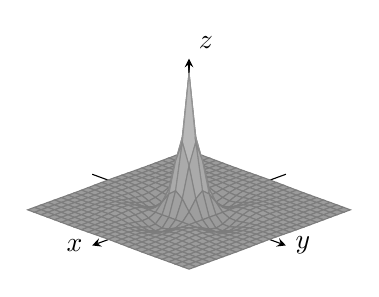
\begin{tikzpicture}[declare function={f(\x,\y)=(cos(deg(\x)))*(cos(deg(\y)))*e^(-sqrt((\x)^2+(\y)^2));}]
\pgfmathsetmacro{\k}{2*pi}
\begin{axis}[view/h=135,small,axis lines=center,colormap={}{gray(0cm)=(0.6);gray(1cm)=(0.8);},xtick={\empty},ytick={\empty},ztick={\empty},xlabel={$x$},ylabel={$y$},zlabel={$z$},enlargelimits=true,xlabel style={anchor=east},ylabel style={anchor=west},zlabel style={anchor=south west}]
\addplot3[surf,domain=-\k:\k,domain y=-\k:\k]{f(x,y)};
\end{axis}
\end{tikzpicture}
\caption{چکور خطہ \عددی{\abs{x}\le \tfrac{3\pi}{2},\,\abs{y}\le \tfrac{3\pi}{2}} پر تفاعل \عددی{z=(\cos x)(\cos y)e^{-\sqrt{x^2+y^2}}} کی زیادہ سے زیادہ قیمت \عددی{1} اور کم سے کم قیمت تقریباً  \عددی{-0.067} ہے۔}
\label{شکل_کثیرالمتغیر_پہاڑی_وادی_الف}
\end{minipage}\hfill
\begin{minipage}{0.45\textwidth}
\centering
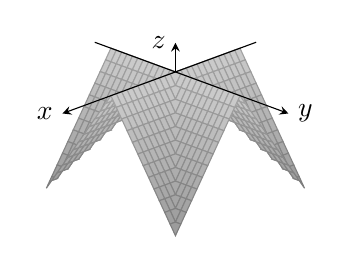
\begin{tikzpicture}[declare function={f(\x,\y)=1/2*(abs(abs(\x)-abs(\y))-abs(\x)-abs(\y));}]
\pgfmathsetmacro{\k}{1}
\begin{axis}[axis on top,view/h=135,small,axis lines=center,colormap={}{gray(0cm)=(0.6);gray(1cm)=(0.8);},xtick={\empty},ytick={\empty},ztick={\empty},xlabel={$x$},ylabel={$y$},zlabel={$z$},enlargelimits=true,xlabel style={anchor=east},ylabel style={anchor=west},zlabel style={anchor=south},xmax=1.5*\k,ymax=1.5*\k, hide z axis]
\addplot3[surf,domain=-\k:\k,domain y=-\k:\k]{f(x,y)};
\addplot3[-stealth]coordinates {(0,0,0)(0,0,0.25)}node[left]{$z$};
\end{axis}
\end{tikzpicture}
\caption{
چکور خطہ \عددی{\abs{x}\le a,\, \abs{y}\le a} پر "تفاعل چھت"   \عددی{z=\tfrac{1}{2}(\abs{\abs{x}-\abs{y}}-\abs{x}-\abs{y})} کی زیادہ سے زیادہ قیمت \عددی{0} اور کم سے کم قیمت \عددی{-a} ہے۔}
\label{شکل_کثیرالمتغیر_پہاڑی_وادی_ب}
\end{minipage}
\end{figure}
\جزوحصہء{تفرقی پرکھ}
واحد متغیری   تفاعل  کا  مقامی  انتہائی نقطہ تلاش کرنے کی  خاطر ہم  ان نقطوں پر نظر رکھتے ہیں جہاں  اس تفاعل کا مماس  افقی ہو۔ان نقطوں پر ہم مقامی مطلق زیادہ سے زیادہ قیمت، مطلق کم سے کم قیمت  یا نقطہ زین  تلاش کرتے ہیں۔ دو متغیری تفاعل \عددی{z=f(x,y)} کے لئے ہم ان نقطوں پر نظر رکھتے ہیں جہاں اس     تفاعل کا مماسی  مستوی  افقی ہو۔  ان نقطوں پر ہم  مقامی مطلق زیادہ سے زیادہ قیمت، مطلق کم سے کم قیمت  یا نقطہ زین  تلاش کرتے ہیں۔ (نقطہ زین پر مزید بات جلد کی جائے گی۔)

\ابتدا{تعریفات}
فرض کریں    خطہ \عددی{R}، جس میں نقطہ \عددی{(a,b)}  پایا جاتا ہو،  میں  تفاعل \عددی{f(x,y)} معین   ہے ۔ تب
\begin{enumerate}[1.]
\item
   اگر کھلا قرص، جس کا مرکز \عددی{(a,b)} ہو،  میں  دائرہ کار  کے تمام نقاط \عددی{(x,y)}پر    \عددی{f(a,b)\ge f(x,y)} ہو تب \عددی{f(a,b)} تفاعل \عددی{f} کا مقامی زیادہ سے زیادہ قیمت   نقطہ ہو گا۔
\item
   اگر کھلا قرص، جس کا مرکز \عددی{(a,b)} ہو،  میں  دائرہ کار  کے تمام نقاط \عددی{(x,y)}پر    \عددی{f(a,b)\le f(x,y)} ہو تب \عددی{f(a,b)} تفاعل \عددی{f} کا  مقامی کم سے کم  قیمت   نقطہ ہو گا۔
\end{enumerate}
\انتہا{تعریفات}
%============

مقامی زیادہ سے زیادہ قیمت نقطہ کو سطح \عددی{z=f(x,y)} پر  پہاڑی  جبکہ مقامی کم سے کم نقطہ کو وادی میں گھاٹی  تصور کیا جا سکتا ہے۔ ایسے نقطوں پر مماسی مستوی  افقی ہوں گے، بشرطیکہ یہ موجود ہوں۔ 

واحد  متغیر تفاعل کی طرح، مقامی انتہا کی تلاش  ایک رتبی تفرقی پرکھ پر منحصر ہو گا۔

\ابتدا{مسئلہ}\شناخت{مسئلہ_کثیرالمتغیر_مقامی_انتہائی_قیمت_یک_رتبی_تفرقی_پرکھ}\موٹا{مقامی انتہائی قیمت کا یک رتبی تفرقی پرکھ}
اگر تفاعل \عددی{f(x,y)} کے دائرہ کار کی اندرونی نقطہ \عددی{(a,b)} پر مقامی زیادہ سے زیادہ یا کم سے کم  قیمت پائی جاتی ہو، اور اگر تفاعل کے  یک رتبی تفرقات  موجود ہوں، تب \عددی{f_x(a,b)=0} اور \عددی{f_y(a,b)=0} ہوں گے۔ 
\انتہا{مسئلہ}
%===================

\ابتدا{ثبوت}
فرض کریں تفاعل \عددی{f} کی دائرہ  کار کے ایک  اندرونی نقطہ \عددی{(a,b)}  پر تفاعل کی مقامی زیادہ سے زیادہ قیمت  پائی جاتی ہے۔ تب
\begin{enumerate}[1.]
\item
مستوی \عددی{y=b} سطح \عددی{z=f(x,y)} کو جس منحنی \عددی{z=f(x,b)} میں قطع کرتا ہے،  نقطہ \عددی{x=a} اس منحنی کے دائرہ کار کا اندرونی نقطہ ہو گا۔
\item
نقطہ \عددی{x=a} پر تفاعل \عددی{z=f(x,b)} متغیر \عددی{x} کے لحاظ سے قابل تفرق ہو گا (اور یہ تفرق \عددی{f_x(a,b)} ہو گا)۔
\item
نقطہ \عددی{x=a} پر تفاعل \عددی{z=f(x,b)} کی مقامی زیادہ سے زیادہ قیمت پائی جائے گی۔  
\item
یوں \عددی{x=a} پر \عددی{z=f(x,b)} کا تفرق صفر ہو گا (مسئلہ \حوالہ{مسئلہ_استعمال_یک_درجی_تفرق_انتہا})۔ چونکہ یہ تفرق \عددی{f_x(a,b)} ہے لہٰذا \عددی{f_x(a,b)=0} ہو گا۔
نقطہ \عددی{x=a}  منحنی  \عددی{z=f(x,b)}  کے دائرہ کار کا اندرونی نقطہ ہو گا۔
\end{enumerate}
تفاعل \عددی{z=f(a,y)}  لیتے ہوئے اسی طرح کی دلیل سے \عددی{f_y(a,b)=0} ثابت کیا جا سکتا ہے۔

یوں مقامی زیادہ سے زیادہ قیمت کے لئے مسئلے  کا  ثابت مکمل ہوتا ہے۔ مقامی کم سے کم قیمت کے لئے مسئلے کا ثبوت آپ سے سوالات میں مانگا  گیا ہے۔
\انتہا{ثبوت}
%==============

ا نقطہ \عددی{(a,b)} پر سطح \عددی{z=f(x,y)}  کے مماسی مستوی  کی مساوات
\begin{align*}
f_x(a,b)(x-a)+f_y(a,b)(y-b)-(z-f(a,b))=0
\end{align*}
میں \عددی{f_x(a,b)=0} اور \عددی{f_y(a,b)=0} پر کرنے سے
\begin{align*}
0\cdot(x-a)+0\cdot(y-b)-z+f(a,b)=0
\end{align*}
یعنی
\begin{align*}
z=f(a,b)
\end{align*}
حاصل ہوتا ہے۔ اس طرح مسئلہ \حوالہ{مسئلہ_کثیرالمتغیر_مقامی_انتہائی_قیمت_یک_رتبی_تفرقی_پرکھ} کہتا ہے  کہ مقامی انتہا پر  یقیناً افقی مماسی مستوی ہو گا، بشرطیکہ اس نقطہ پر مماسی مستوی موجود ہو۔

واحد متغیر تفاعل کی صورت کی  طرح، مسئلہ \حوالہ{مسئلہ_کثیرالمتغیر_مقامی_انتہائی_قیمت_یک_رتبی_تفرقی_پرکھ} کہتا ہے کہ تفاعل \عددی{f(x,y)} کی  انتہائی قیمت صرف اور صرف   درج ذیل  نقطوں پر پائی جا سکتی ہے:
\begin{enumerate}[1.]
\item
اندرونی نقاط جہاں \عددی{f_x=f_y=0} ہو،
\item
اندرونی نقاط جہاں \عددی{f_x} اور \عددی{f_y} میں سے ایک یا دونوں غیر موجود ہوں،
\item
تفاعل کے دائرہ کار کے سرحدی نقاط۔
\end{enumerate}

\ابتدا{تعریف}
تفاعل \عددی{f(x,y)} کے دائرہ کار  کا     وہ اندرونی نقطہ  جہاں \عددی{f_x} اور \عددی{f_y} دونوں  صفر ہوں یا جہاں    \عددی{f_x} اور \عددی{f_y}میں سے ایک یا  دونوں غیر موجود ہوں، \عددی{f} کا \اصطلاح{ نقطہ فاصل}\فرہنگ{نقطہ!فاصل}\حاشیہب{critical point}\فرہنگ{point!critical} ہو گا۔
\انتہا{تعریف}
%====================

اس طرح تفاعل \عددی{f(x,y)}  کی انتہائی قیمتیں صرف  نقاط فاصل اور سرحدی نقاط  پر پائی جائیں گی۔ واحد متغیر  کے قابل تفرق تفاعل کی طرح، ضروری نہیں کہ ہر نقطہ فاصل پر مقامی انتہا   ہو۔ واحد متغیر کے قابل تفرق تفاعل کا نقطہ تصریف  ممکن ہے۔ دو متغیرات کے قابل تفرق تفاعل  کا نقطہ زین ممکن ہو گا۔  

\ابتدا{تعریف}
  نقطہ فاصل  \عددی{(a,b)} پر اس صورت قابل تفرق تفاعل \عددی{f(x,y)} کا \اصطلاح{ نقطہ زین}\فرہنگ{نقطہ!زین}\حاشیہب{saddle point}\فرہنگ{point!saddle}پایا جائے گا جب ہر کھلے  قرص میں، جس  کا مرکز \عددی{(a,b)} ہو،   ایسے  دائرہ کاری  نقاط \عددی{(x,y)} پائے جاتے ہوں جن پر  \عددی{f(x,y)>f(a,b)} ہو، اور ایسے دائرہ کاری  نقاط \عددی{(x,y)} پائے جاتے ہوں جن پر  \عددی{f(x,y)<f(a,b)}ہو۔ سطح \عددی{z=f(x,y)} پر مطابقتی نقطہ  \عددی{(a,b,f(a,b))}  اس  سطح کا نقطہ زین کہلاتا ہے۔ 
\انتہا{تعریف}
%==================
